\documentclass[10pt]{beamer}
\usepackage[linesnumbered,algoruled,boxed,lined]{algorithm2e}
\usetheme{metropolis}
\usepackage{appendixnumberbeamer}
\usepackage[utf8]{vietnam}
\usepackage{booktabs}
\usepackage[scale=2]{ccicons}

\usepackage{pgfplots}
\usepgfplotslibrary{dateplot}

\usepackage{xspace}
\newcommand{\themename}{\textbf{\textsc{metropolis}}\xspace}
\newcommand{\SubItem}[1]{
    {\setlength\itemindent{15pt} \item[-] #1}
}
\usepackage{listings}
\usepackage{lstautogobble} % Provides autogobble, which is useful to remove indentation based on first line

\lstset{ %
  language=bash,
%  numbers=left,
  numberstyle=\tiny,
  stepnumber=1,
  numbersep=5pt,
  breaklines=true,
  autogobble=true, % Removes indentation based on first line
}

\title{Nghiên cứu phát triển kỹ thuật đếm\\ số phần tử  trên dòng dữ liệu}
% \subtitle{Nghiên cứu phát triển kỹ thuật đếm số phần tử \\ \hspace{2.4cm} trên dòng dữ liệu}
\date{Người hướng dẫn khoa học: \hspace{0.5cm}PGS. TS. THOẠI NAM}
\author{Học viên: Lê Anh Quốc \hspace{1cm} ID: 2070428}
%\institute{\today}
\titlegraphic{\hfill
\includegraphics[height=1.5cm]{hcmut.png}}

\begin{document}

\maketitle

\begin{frame}{Outline}
  \setbeamertemplate{section in toc}[sections numbered]
  \tableofcontents[hideallsubsections]
\end{frame}

\section{Giới thiệu}

\begin{frame}[fragile]{Giới thiệu}

\begin{itemize}
  \item Ứng dụng và dịch vụ trực tuyến đóng vai trò quan trọng trong cuộc sống hiện đại.
  \item DAU (\textbf{Daily Active Users}) là chỉ số quan trọng để đánh giá hiệu quả hoạt động của các ứng dụng và dịch vụ này.
  \item Theo dõi DAU giúp:
  \SubItem{Đánh giá mức độ tương tác và quan tâm của người dùng.}
  \SubItem{Đo lường hiệu quả của chiến dịch marketing và quảng cáo.}
  \SubItem{Hỗ trợ ra quyết định kinh doanh.}
  \item Thách thức:
  \SubItem{Đếm DAU trên dữ liệu lớn và tốc độ truy cập cao.}
  \SubItem{Tổng hợp DAU từ nhiều nguồn dữ liệu khác nhau.}
\end{itemize}
\end{frame}

\section{Các công trình nghiên cứu liên quan}
\begin{frame}{Các công trình nghiên cứu liên quan}
\begin{itemize}
	\item Philippe Flajolet, Éric Fusy, Olivier Gandouet, and Frédéric Meunier\\ LogLog Counting of Large Cardinalities, 2003 \cite{durand2003loglog}: 
	\SubItem{Thuật toán ước lượng số lượng phần tử với độ chính xác cao và sử dụng ít bộ nhớ.}
	\item Philippe Flajolet, Éric Fusy, Olivier Gandouet, and Frédéric Meunier\\ HyperLogLog: The Analysis of a Near-Optimal Cardinality Estimation Algorithm, 2007 \cite{flajolet2007hyperloglog}: 
	\SubItem{là một cải tiến từ LogLog, thuật toán này có khả năng ước lượng số lượng phần tử lớn hơn $10^9$ với sai số khoảng 2\% chỉ dụng 1.5 kilobytes bộ nhớ, đồng thời có khả năng song song hoá tối ưu và thích nghi với mô hình cửa sổ trượt (sliding window).}
	\item Stefan Heule, Marc Nunkesser, Alexander Hall\\ HyperLogLog in Practice: Algorithmic Improvements for Practical Cardinality Estimation Deployments, 2017 \cite{heule2013hyperloglog}: 
	\SubItem{Phiên bản nâng cấp của HyperLogLog với độ chính xác cao hơn và yêu cầu bộ nhớ ít hơn.}
\end{itemize}
\end{frame}

\section{Phát biểu bài toán}
\begin{frame}[fragile]{Phát biểu bài toán}
  \begin{itemize}
    \item \textbf{Bài toán 1:} Phát triển thuật toán để ước lượng số lượng phần tử (cardinality estimation) trong một khoảng thời gian trên một dòng dữ liệu (data stream).
    \item \textbf{Bài toán 2:} Mở rộng thuật toán để ước lượng số lượng phần tử trong một khoảng thời gian trên nhiều dòng dữ liệu.
  \end{itemize}
\end{frame}
\section{Mục tiêu, đối tượng và giới hạn nghiên cứu}

\begin{frame}{Mục tiêu}
  \begin{itemize}
      \item Phát triển kỹ thuật đếm số lượng phần tử hiệu quả, có chính xác cao trên dòng dữ liệu.
      \item Nâng cao hiệu suất xử lý dữ liệu lớn, đáp ứng nhu cầu ngày càng tăng trong kỷ nguyên số.
      \item Thực hiện, phân tích kết quả thí nghiệm, rút ra kết luận và đề xuất hướng nghiên cứu tiếp theo.
      \item Đóng góp vào sự phát triển của công nghệ dữ liệu lớn, mở ra tiềm năng ứng dụng trong nhiều lĩnh vực.
  \end{itemize}
\end{frame}

\begin{frame}{Giới hạn, đối tượng nghiên cứu}
  \textbf{Đối tượng nghiên cứu}:
    \begin{itemize}
        \item Dòng dữ liệu dạng \textbf{văn bản} có chứa nhiều phần tử cần đếm.
        \SubItem{userID, IP address, words, etc}
        \item Các kỹ thuật đếm số lượng phần tử.
    \end{itemize}
  \textbf{Giới hạn}:
  \begin{itemize}
    \item Nghiên cứu kỹ thuật đếm số lượng phần tử trên \textbf{dòng dữ liệu} dạng văn bản.
    \item Các kỹ thuật được đề xuất và triển khai có thể chưa áp dụng 
    được cho tất cả các loại dữ liệu.
    \SubItem{Hình ảnh, âm thanh ...}
  \end{itemize}
  
\end{frame}

\section{Cơ sở lý thuyết}

\begin{frame}[fragile]{Cơ sở lý thuyết}
  \textbf{LogLog Algorithm}
  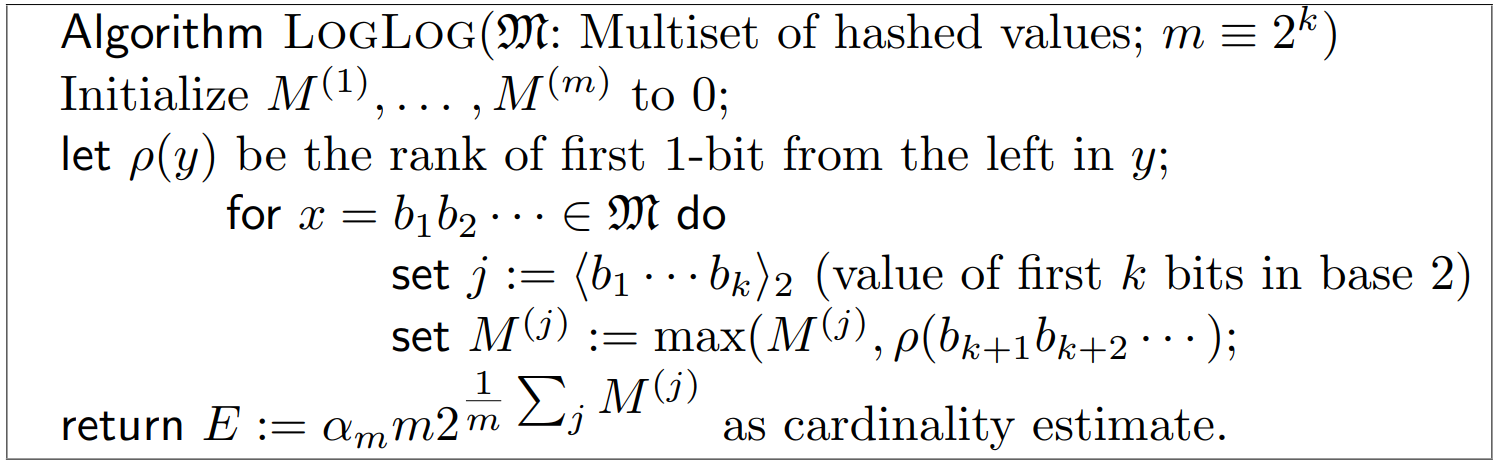
\includegraphics[scale=0.35]{loglog.png}
  \indent Sai số tiêu chuẩn $\delta$ của thuật toán \textit{LogLog}:
\[\delta \approx \frac{1.3}{\sqrt{m}}\]
\begin{itemize}
  \item $m = 256$, $\delta \approx 8\%$
  \item $m = 1024$, nó giảm xuống còn khoảng 4\%.
\end{itemize}
\end{frame}

\begin{frame}{HyperLogLog algorithm}
\begin{itemize}
	\item Đã được đề xuất bởi Philippe Flajolet, Eric Fusy, Olivier Gandouet và 
  Frederic Meunier vào năm 2007 \cite{flajolet2007hyperloglog}.
  \item Sử dụng hàm băm 32-bit và hàm đánh giá có các sửa lỗi \textbf{bias} khác nhau.
  \item Xử lý các định lượng lên đến $10^9$ với một hàm băm 32-bit đơn lẻ $h$ chia tập dữ liệu thành $m = 2^p$ tập con, với $p \in 4...16$.
  \item Sử dụng trung bình điều hoà (\textbf{hamonic} mean) thay vì sử dụng trung bình hình học (geometric mean) như phiên bản gốc LogLog

\end{itemize}

\end{frame}
\begin{frame}{HyperLogLog algorithm}
  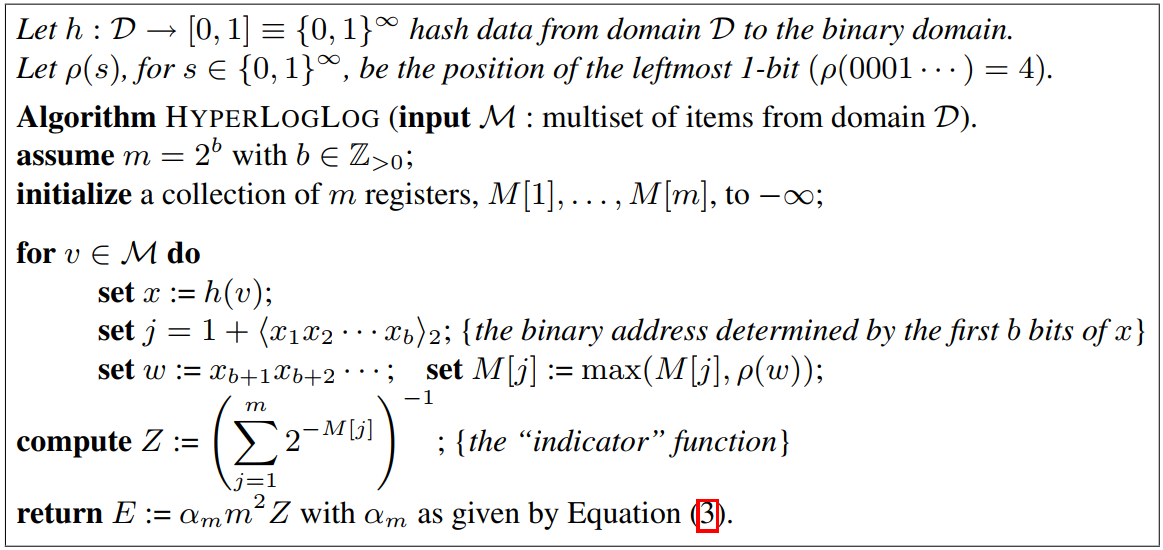
\includegraphics[scale=.468]{raw_hll.png}
  \indent Với $\alpha_m$:
  \[
      \alpha_m = \left(m\int_0^\infty\left(\log_2\left(\frac{2+x}{1+x}\right)\right)^m\text{dx}\right)^{-1} \hspace{1cm}(3)  
  \]
\end{frame}

\begin{frame}{HyperLogLog algorithm}
\begin{itemize}
	\item Tương tự LogLog, sai số tiêu chuẩn $\delta$: \[\delta \approx \frac{1.04}{\sqrt{m}}.\]
	\item Yêu cầu bộ nhớ không tăng tuyến tính theo số lượng phần tử, 
  $m = 2^p$ bộ đếm, bộ nhớ cần thiết là:
  \[\lceil\log_2\left(M + 1 - p\right)\rceil\cdot2^p \text{ bits }\]
  \item Ví dụ, \textbf{Redis} duy trì cấu trúc dữ liệu \textit{HyperLogLog} của \textbf{12 KB} để xấp xỉ các định lượng $\delta \approx 0.81.\%$.
  \SubItem{$\log_2(64 + 1 - 14)*2^{14}$, sử dụng hàm băm 64-bit và p = 14}
  \SubItem{$\delta \approx \frac{1.04}{\sqrt{2^{14}}} = 0.008125$}
\end{itemize}
\end{frame}

\begin{frame}{HyperLogLog: các thư viện và công cụ nổi bật }
  \begin{itemize}
    \item \textbf{Apache DataSketches:} một thư viện Java cung cấp các thuật toán xác suất và thống kê. Được sử dụng rộng rãi trong các hệ thống Big Data như 
    Apache Druid, Apache Kafka và Apache Hive.
    \item \textbf{Redis:} hệ thống lưu trữ dữ liệu dạng key-value phổ biến, cung cấp 
    cấu trúc dữ liệu HyperLogLog tích hợp sẵn. Sử dụng các lệnh như PFADD, PFCOUNT 
    và PFMERGE để làm việc với HLL.
    \item \textbf{Google BigQuery:} sử dụng HyperLogLog++ cho các chức năng thống kê và phân tích dữ liệu lớn.
    \item \textbf{PostgreSQL:} Extension postgreSQL-hll giúp thực hiện các truy vấn với số lượng phần tử duy nhất một cách hiệu quả.
    \item \textbf{Amazon Redshift:} hỗ trợ HyperLogLog để tối ưu hóa các truy vấn thống kê và giảm thiểu dung lượng bộ nhớ cần thiết.
    \item \textbf{Apache Flink:} một nền tảng xử lý luồng dữ liệu phân tán, 
    có tích hợp HyperLogLog để xử lý các phép tính phức tạp trên dữ liệu luồng.
  \end{itemize}
\end{frame}

\begin{frame}{Ví dụ: Redis (1/3)}
Redis là một hệ thống lưu trữ dữ liệu dạng key-value phổ biến và hỗ trợ nhiều cấu trúc dữ liệu mạnh mẽ, trong đó có HyperLogLog. Redis cung cấp các lệnh chuyên biệt để làm việc với HyperLogLog, bao gồm PFADD, PFCOUNT và PFMERGE.\\
\textbf{Các lệnh cơ bản của HyperLogLog trong Redis:}
  \begin{itemize}
    \item \textbf{PFADD:} Thêm các phần tử vào HyperLogLog.
    \item \textbf{PFCOUNT:} Ước lượng số phần tử duy nhất trong HyperLogLog.
    \item \textbf{PFMERGE:} Hợp nhất nhiều HyperLogLog thành một.
  \end{itemize}
\end{frame}

\begin{frame}{Ví dụ: Redis (2/3)}
Giả sử chúng ta có một ứng dụng web và muốn theo dõi số lượng người dùng duy nhất truy cập vào website mỗi ngày.\\
\textbf{Các lệnh cơ bản của HyperLogLog trong Redis:}
  \begin{itemize}
    \item \textbf{Cài đặt Redis:} 
   	\SubItem{sudo apt-get update}
   	\SubItem{sudo apt-get install redis-server}
    \item \textbf{Khởi động Redis server:} 
    \SubItem{redis-server}   
    \item \textbf{Kết nối tới Redis:}
    \SubItem{redis-cli}
   \end{itemize}
\end{frame}

\begin{frame}[fragile]{Ví dụ: Redis (3/3)}
\begin{itemize}
	\item \textbf{Thêm người dùng}:
	\begin{lstlisting}
PFADD unique_visitors:2024-05-25T08 user1 user2 user3
PFADD unique_visitors:2024-05-25T08 user2 user4
PFADD unique_visitors:2024-05-25T09 user5 user6
PFADD unique_visitors:2024-05-25T10 user1 user7
\end{lstlisting}
\item \textbf{Ước lượng số người dùng trong giờ 08:00 ngày 2024-05-25}:
	\begin{lstlisting}
PFCOUNT unique_visitors:2024-05-25T08
\end{lstlisting}
\item \textbf{Giả sử chúng ta muốn hợp nhất dữ liệu người dùng duy nhất từ ba giờ khác nhau (08:00, 09:00, và 10:00).}:
	\begin{lstlisting}
PFMERGE unique_visitors:2024-05-25:morning unique_visitors:2024-05-25T08 unique_visitors:2024-05-25T09 unique_visitors:2024-05-25T10
PFCOUNT unique_visitors:2024-05-25:morning
\end{lstlisting}
\end{itemize}
\end{frame}

\begin{frame}[fragile]{Cách HyperLogLog lưu trữ dữ liệu trong Redis}
Redis sử dụng "sparse representation" cho các bộ đếm nhỏ và "dense representation" cho các bộ đếm lớn hơn.\\
Dung lượng bộ nhớ phụ thuộc vào số lượng thanh ghi (registers), 
và mỗi thanh ghi lưu trữ thông tin về vị trí của bit đầu tiên là 1 
trong chuỗi băm.\\
\vspace{0.2cm}
\textbf{Số lượng thanh ghi (m)}:
\begin{itemize}
	\item $m = 2^p$, trong đó p là số bit để xác định số thanh ghi.
	\item Giá trị mặc định p trong Redis là \textbf{14} => có $2^{14} = 16384$ thanh ghi.
\end{itemize}
\textbf{Dung lượng bộ nhớ cần thiết}
\begin{itemize}
	\item Mỗi thanh ghi cần \textbf{6 bit} để lưu trữ vị trí của bit đầu tiên là 1.
	\item Tổng dung lượng bộ nhớ cần thiết cho HyperLogLog trong Redis có thể 
  tính theo công thức (với m = 16384 thanh ghi):\\ 
	Memory = 16384 x 6 bits = 98304 bits = 12288 bytes = \textbf{12 KB}
\end{itemize}
\end{frame}

\begin{frame}[fragile]{Tính toán dung lượng cần thiết cho nhiều tập hợp HLL}
Nếu bạn muốn lưu trữ nhiều tập hợp HyperLogLog trong Redis, ví dụ như 
theo dõi số người dùng duy nhất theo giờ, cần nhân dung lượng bộ nhớ 
của một tập hợp HLL với số lượng tập hợp bạn có.\\
Giả sử bạn muốn lưu trữ dữ liệu người dùng duy nhất cho mỗi giờ trong 
một ngày (24 giờ):\\
\begin{center}
  Total Memory = 12 KB x 24 = \textbf{288 KB}
\end{center} 
Nếu bạn muốn lưu trữ dữ liệu theo từng giờ cho nhiều ngày, bạn chỉ cần 
nhân thêm số lượng ngày:
\begin{center}
  Total Memory for 30 days = 288 KB/day × 30 = 8640 KB = \textbf{8.64 MB}
\end{center} 
\end{frame}

\section{Phương pháp thực hiện}
\begin{frame}[fragile]{Bài toán 1}
Phát triển thuật toán để ước lượng số lượng phần tử (cardinality estimation) trong 
một khoảng thời gian trên một dòng dữ liệu (data stream): 

\begin{itemize}
  \item Bước 1: Xác định khoảng thời gian
  Đầu tiên, chúng tôi sẽ xác định khoảng thời gian mà chúng tôi muốn đếm số lượng 
  phần tử. Ví dụ, mỗi giờ hoặc mỗi phút.
  \item Bước 2: Lưu trữ HyperLogLog
  Tiếp theo, chúng tôi sẽ lưu trữ cấu trúc HyperLogLog cho mỗi khoảng thời gian. 
  Cấu trúc dữ liệu sẽ bao gồm cặp $\left< T, HLL_1\right>$, trong đó $T$ là 
  thời điểm đại diện cho khung thời gian cụ thể.
  \item Bước 3: Sử dụng kết quả
  Cuối cùng, khi cần, chúng tôi có thể truy vấn và sử dụng kết quả từ các cấu trúc 
  HyperLogLog lưu trữ theo khung thời gian để ước lượng số lượng phần tử trong 
  mỗi khoảng thời gian.
\end{itemize}
\end{frame}
\begin{frame}[fragile]{Bài toán 2}
%   Mở rộng thuật toán để ước lượng số lượng phần tử trong một khoảng thời gian trên nhiều dòng dữ liệu:\\
% \vspace{0.1cm}
%   \textit{ Ví dụ khi chúng ta cần biết có bao nhiêu người dùng đã đăng nhập vào hệ thống vào ngày hôm qua, do dữ liệu người dùng được lưu ở trên nhiều hệ thống như web, application và cũng như trên các bộ phận khác nhau của doanh nghiệp. Khi đó chúng ta sẽ có nhiều nguồn dữ liệu khác nhau và cần một thuật toán để kết hợp các nguồn dữ liệu này để tổng hợp cho ra ước lượng
%   số lượng cuối cùng.}
  \begin{itemize}
    \item Mở rộng thuật toán để ước lượng số lượng phần tử trong 
    một khoảng thời gian trên nhiều dòng dữ liệu:
    \SubItem{Ví dụ khi chúng ta cần biết có bao nhiêu người dùng 
    đã đăng nhập vào hệ thống vào ngày hôm qua, do dữ liệu người 
    dùng được lưu ở trên nhiều hệ thống như web, application và 
    cũng như trên các bộ phận khác nhau của doanh nghiệp.} 
    \item Bước 1: Lưu trữ dữ liệu
    \SubItem{Lưu trữ dữ liệu theo khung thời gian $\left< T, HLL\right>$}
    \item Bước 2: Tổng hợp HLL từ các dữ liệu từ nhiều nơi khác nhau:\\
    $\left< T, HLL_1\right>, \left< T, HLL_2\right>,...,\left< T, HLL_N\right>$\\
    \SubItem{$T$ là khoảng thời gian cần tổng hợp} \\
    \SubItem{$HLL_1$ là dữ liệu HyperLogLog trong khoảng thời gian}
    \item Bước 3: Ước lượng số phần tử
\end{itemize}

\end{frame}
\section{Kế hoạch triển khai}
\begin{frame}{Kế hoạch triển khai}
\begin{tabular}{ |c|c|l| }
    \multicolumn{3}{}{} \\ \hline
    \# & Tuần & Nội dung công việc \\ \hline
    1 & 1 - 2 &\vtop{\hbox{\strut Bài báo liên quan mới nhất và bổ sung cơ sở lý thuyết}\hbox{\strut về các kỹ thuật ước lượng số lượng trên dòng dữ liệu}}\\
    \hline
    2 & 3 - 4 &\vtop{\hbox{\strut Thu thập dữ liệu, chuẩn hoá và tiền xử lý. Hiện thực}\hbox{\strut bài toán 1 ước lượng số lượng phần tử trên dòng dữ liệu}}\\
    \hline
    3 & 5 - 6 &\vtop{\hbox{\strut Mở rộng để ước lượng số lượng phần tử trên }\hbox{\strut nhiều dòng dữ liệu. Đánh giá hiệu suất và độ chính xác.}}\\
    \hline
    4 & 7 - 8 &\vtop{\hbox{\strut Phân tích và so sánh kết quả, đánh giá ưu nhược điểm.}\hbox{\strut Đề suất phương pháp tối ưu hiệu suất và độ chính xác.}}\\
    \hline
    5 & 9 - 10 &\vtop{\hbox{\strut Ứng dụng kết quả nghiên cứu.}\hbox{\strut Đề suất hướng phát triển và nghiên cứu tiếp theo.}}\\
    \hline
    6 & 11 - 12 &\vtop{\hbox{\strut Đề xuất và đánh giá các giải pháp}}\\
    \hline
    7 & 1 - 14 & Tổng hợp kết quả và viết báo cáo \\
    \hline
\end{tabular}
\end{frame}

\begin{frame}{Nội dung dự kiến của luận văn}
  \textbf{Chương 1: Giới thiệu}. Tầm quan trọng của việc phát triển kỹ thuật đếm 
  số phần tử trên dòng dữ liệu trong ngữ cảnh 
  dữ liệu lớn.\\
  \textbf{Chương 2: Các công trình nghiên cứu liên quan.} Các công trình nghiên cứu 
  liên quan, phương pháp giải quyết vấn đề. Đánh giá tính khả thi của đề tài.\\
  \textbf{Chương 3: Kiến thức nền tảng.} Giới thiệu về tính chất, phương pháp
  truy vấn và xử lý trên dòng dữ liệu. Giới thiệu về HyperLogLog và nguyên lý 
  hoạt động và đánh giá hiệu suất, độ chính xác trên dòng dữ liệu.\\
  \textbf{Chương 4: Hiện thực và thử nghiệm. } Trong chương này sẽ trình bày chi tiết 
  cách thức hiện thực của từng thuật toán.\\
  \textbf{Chương 5: Kết quả và đánh giá.} Trong chương này sẽ nêu ra các kết quả 
  đạt được của các kỹ thuật, cũng như phương pháp đánh giá dựa trên kết quả thực nghiệm.\\
  \textbf{Chương 6: Kết luận.} Đánh giá ưu điểm và nhược điểm của mô hình và 
  đề xuất hướng nghiên cứu phát triển kỹ thuật đếm số phần tử trong tương lai.
\end{frame}

\begin{frame}[fragile]{Tài liệu tham khảo}
  \bibliography{ref}
  \bibliographystyle{ieeetr}
\end{frame}

\begin{frame}[fragile]
  \begin{center}
    \LARGE \textbf{Q \& A}
  \end{center}
\end{frame}

\begin{frame}[fragile]
  \begin{center}
    \LARGE \textbf{Chân thành cảm ơn!}
  \end{center}
\end{frame}

\end{document}
